%
		\subsection{Bohm Criteria}\label{sec:bohmcriteria}
%
			In~\autoref{sec:sheathphysics} the behaviour of charge particle densities inside the plasma sheath has been discussed. In contrast to the discharge volume, those densities do not satisfy the quasi-neutrality condition in a distance of $d$ from the wall any more. Though we know that the sheath is a spatially restricted area around electrostatic floating surfaces, a physical law concerning this circumstance has not been derived here. So the question ensues, why the area of electron depletion does not extend further into the discharge volume.\\
			To answer this question, one has to take a look at a substitutional system. This will be a, likewise mechanical, one-body extremal problem of a point mass. In this case only kinematic potentials with inverted parabolic maxima are of interest. Therefore, in this unstable equilibrium, a small pertubation culminates into a large force on the test body.\\
			To see the quality of this example, one has to take a look at the second order differential equation of the afore-mentioned mechanical problem and the electrostatic \emph{Poisson's equation} (see~\autoref{equ:pseudo}).
%
			\begin{align} 
				m\frac{\diff^{2}\vec{r}}{\diff t^{2}}=-\frac{\diff V}{\diff\vec{r}}%
						\quad\Leftrightarrow\quad%
						\Delta_{\vec{r}}\Phi=-\frac{\diff\Psi}{\diff\Phi}=f{\left(\Phi\right)}%
						\hspace{-0.33cm}\overset{\text{Poisson's}}{\overset{\mid}{=}}\hspace{-0.33cm}%
						\frac{\rho}{\varepsilon\ix{0}}%
				\label{equ:pseudo}
			\end{align}
%
			\begin{figure}[!b]
				\centering%
				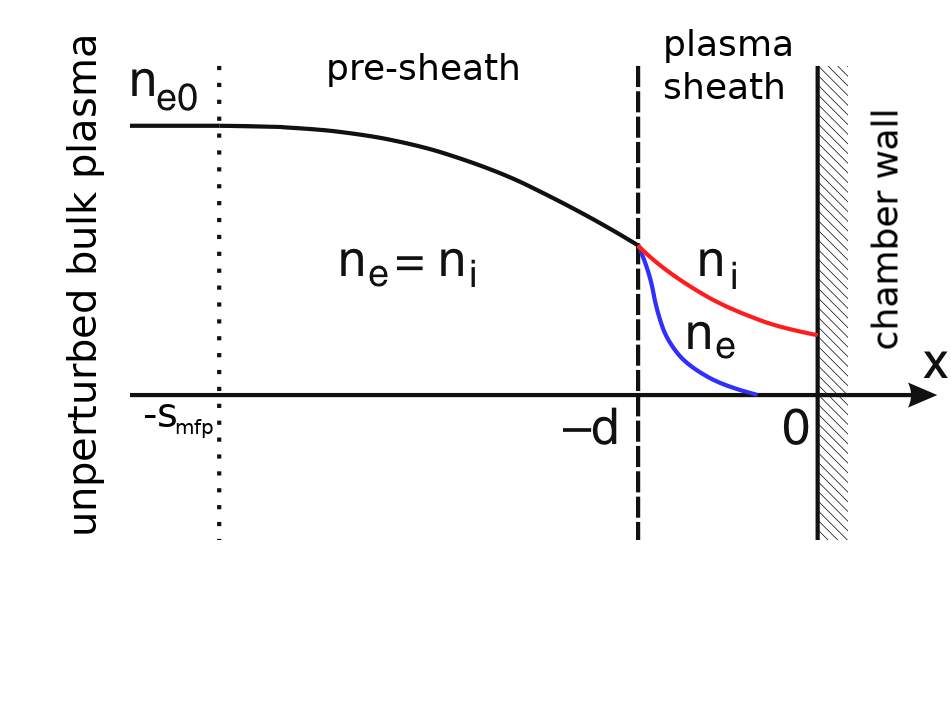
\includegraphics[width=0.6\textwidth]{figures/sheath_piel.png}%
				\caption{%
				One dimensional density profiles as a function of the distance to a floating wall. Note the exponential decrease of the electron density $n\ix{e}$ from the sheath border towards the presumably negatively charged wall. Densities allready reach approximately $0,66n\ix{e,0}$ inside the pre-sheath.~\cite{Piel10}}\label{fig:sheath_piel}
			\end{figure}
%
			For an instability, the force on the test body must increase with the distance from the equilibrium, hence the~\autoref{equ:inequality} is used to calculate the exact velocity at which an ion is entering the sheath. This results in the first \emph{Bohm criteria}.
%
			\begin{align}
				0>\left.\frac{\diff^{2}\Psi}{\diff\Phi^{2}}\right|_{\Phi=0}%
				\overset{\text{\autoref{equ:pseudo}}}{\overset{\mid}{=}}%
						\left.\frac{\diff}{\diff\Phi}\left(\frac{n\ix{e}\left(x\right)-n\ix{i}%
						\left(x\right)}{\varepsilon\ix{0}}\right)\right|_{\Phi=0}&%
						\frac{en\ix{e}\left(-d\right)}{\varepsilon\ix{0}}\left(\frac{e}%
						{k\ix{b}T\ix{e}}-\frac{e}{m\ix{i}v\ix{i,0}^{2}}\right)%
				\label{equ:condition}\\[10pt]%
				\Rightarrow\quad%
				v\ix{i,0}\ge v\ix{i,B}=\sqrt{\frac{k\ix{B}T\ix{e}}{m\ix{i}}}&%
				\label{equ:inequality}
			\end{align}
%	
			Analoguos you can define the so called \emph{Mach number} $M=v\ix{i,0}/v\ix{i,B}$, where $v\ix{i,B}$ denotes the \emph{Bohm velocity}.\\
			Now, to understand why the sheath does not extend further than a fixed distance $d$ from the discharge boundary, the particle movement has to be investigated on a smaller scale. As seen above, there is an electric field in the \emph{pre-sheath} that accelerates the ions to $v\ix{i,B}$. In addition, quasi-neutrality is still satisfied here:
%
			\begin{align}
				n\ix{i}\left(x\right)=n\ix{i,0}\exp\left(\frac{e\Phi\left(x\right)}{k\ix{B}T\ix{e}}\right)%
				=n\ix{e}\left(x\right)\,\,.%
				\label{equ:quasineutral}
			\end{align}
%
			Still, $\Phi{\left(x\right)}$ is the potential inside the pre-sheath from~\autoref{sec:sheathphysics} and $n\ix{i,0}$ the unperturbed density from the plasma \emph{bulk}. A greater part of the ion transport process in this area is governed by collisions with neutral gas particles, hence the velocity distribution function with the collision frequency $\nu\ix{n,i}$ has to be rewritten:
%
			\begin{align}
				\frac{\diff v\ix{i}}{\diff x}=\frac{\nu\ix{n,i}v\ix{i}^{2}}{v\ix{B}^{2}-v\ix{i}^{2}}\quad.%
				\label{equ:distribution}
			\end{align}
%
			From the singularity in~\autoref{equ:distribution} at $v\ix{i}=v\ix{B}$ and the knowledge of $\Phi(x)$ at the wall, one can calculate the sheath thickness $d$. Furthermore, ions with velocities smaller than the Bohm velocity are being accelerated inside the pre sheath. According to~\autoref{equ:inequality} velocities greater than $v\ix{B}$ are not allowed here. This is, together with~\autoref{equ:distribution} the reason why the ion velocity is exactly $v\ix{B}$ at the boundary of the plasma sheath and thus a positive space-charge ensues.
%
			\begin{align}
				M\ge1%
				\Leftrightarrow%
				v\ix{i}(-d)\ge v\ix{B}%
				\label{equ:bohmcriteria2}
			\end{align}
%
			Conclusively, at the sheath boundary~\autoref{equ:bohmcriteria2} is satisfied.\\
			At $x=-d$, both negative and positive charge density decreased to $n\ix{i}=n\ix{e}\approx\SI{0.66}n\ix{e,0}$ (see~\autoref{fig:sheath_piel}), where the potential is approximately $-k\ix{B}T\ix{e}/2e$ because of the currents onto the wall.\\
			In summarization, the plasma does not `see' its sheath, because the ion dynamic discussed before is spatially restricted. The sheath only develops where there is electron depletion or an externally applied, negative potential.
